\documentclass[
%*********************************************
%* Paper type (letterpaper)                  *
%*********************************************
    a4paper,
%   letterpaper,
%   a5paper,
%   b5paper,
%   executivepaper,
%   legalpaper,
%
%*********************************************
%* Font size (10pt)                          *
%*********************************************
%   10pt,
    11pt,
%   12pt,
%
%*********************************************
%* Paging (document dependent)               *
%*********************************************
    oneside,
%   twoside,
%
%*********************************************
%* Equation alignment (center)               *
%*********************************************
%   fleqn,                  %placerer fomlerne i venstre siden istedet for centreret.
%   leqno,                  %Placerer formelnummereringen på venstre side (istedet for højre)
%
%*********************************************
%* Chapter positioning (document dependent)  *
%*********************************************
    openany,                %openany starter chapters på næstkommende side.
%   openright,
%
%*********************************************
%* Language (none)                           *
%*********************************************
%    english]
   danish]
%
%*********************************************
%* Document type (none)                      *
%*********************************************
%   {book}
    {article}
%   {slides}
%   {report}


%*********************************************
%* Userpackages                              *
%*********************************************
\usepackage[danish]{babel}
%\usepackage{t1enc}          %Bruges til sprog oa.
\usepackage[latin1]{inputenc}
\usepackage{amsfonts}
\usepackage{mathrsfs}
%\usepackage[xdvi]{epsfig}
%\usepackage{ifthen}
%\usepackage{latexsym}
%\usepackage{theorem}
\usepackage[dvips]{graphicx}       %Used when including .eps (graphics) files
%\usepackage{varioref}
%\usepackage{epic}
%\usepackage{eepic}
%\usepackage{rotfloat}
%\usepackage{multicol}
%\usepackage{wrapfig}
%\usepackage{syntonly}          %Use this to check for proper syntax, makes output file.
%\syntaxonly                %Use this to check for proper syntax, makes NO output file.
\usepackage{verbatim}          %Used when to include an unformatted ASCII file
%\usepackage{fancyhdr}
%\usepackage{layout}
%\usepackage{float}
%\usepackage{makeidx}          %Used when making an index in the document
\usepackage{calc}              %Used if you wanna use cm, mm, ex etc. instead of pt

%%
%% For code syntax highliting
%%
%\usepackage{color}
%\usepackage{alltt}

\pagestyle
%*********************************************
%* Header / footer configuration (none)      *
%*********************************************
    {plain}                 %Writes page number in footer, header is empty.
%   {headings}
%   {empty}                 %Makes no header or footer
%   {myheadings}
%   {fancy}



%*********************************************
%* Extra pagelayout    (se s. 110)           *
%*********************************************
%\hoffset   =   -0.5cm %Venstremargin
%\voffset   =   0pt
%\evensidemargin=   0pt
%\oddsidemargin =   0pt %Ekstra venstremargin til dobbeltsider
%\topmargin =   -2cm
%\headheight    =   0pt
%\headsep   =   0pt
%\textheight = 690pt
%\textwidth =   480pt
%\marginparsep  =   0pt
%\marginparwidth=   0pt
%\footskip  =   0pt
%\marginparpush =   0pt
%\paperwidth    =   597pt
%\paperheight   =   845pt

%\makeindex

%\parskip   =   1ex
%\parindent =   0em
%\baselineskip  =   2ex

%\underlineheadings

\title{LPC �velse}
%
\author{Mikkel Gravgaard - 20043246\\Bent Bisballe Nyeng - 20001467}

\markboth{}{}
%*********************************************
%*                start of                   *
%*              -=DOCUMENT=-                 *
%*********************************************
\begin{document}
\maketitle
\tableofcontents 
Vi ønsker i denne øvelse at implementere billedkomprimering ved hjælp af de teknikker som benyttes i JPEG, nemlig kvantisering af en frekvensmatrice samt Huffman-kodning.

Vi ønsker at konstruere vores program således at det er muligt for brugeren at eksperimentere med forskellige kvantiseringsindstillinger.


\section{Brugervejledning}
\subsection*{Quality}
\begin{verbatim}
Usage: ./lpc [options] inputfile outputfile
Options:
  -w  --windowsize ms   Set the window size to ms (default 20).
  -c  --coefficients c  Set the number of coefficients to use with 
                        the lpc to c (default 20).
  -t  --threshold t     Set the pitched/unpitched threashold to t 
                        (default 0.065).
  -v  --volume v        Set volume multiplyer to v (default 1.000).
  -o  --overlap         Make windows overlap 50
  -h, --help            Print this message and exit.
\end{verbatim}

% -*- coding: latin-1 -*-
\section{LPC-analyse og syntese}
Til LPC-analysen har vi benyttet RT\_LPC som en blackbox. M�den hvorp� LPC-analysen foreg�r er beskrevet p� http://wiki.cs.princeton.edu/index.php/RT\_LPC.

Ligesom ved analysedelen af LPC, benytter vi ogs� RT\_LPC til at syntetisere talen, s�ledes at vi blot giver de ved analysen fundne koefficienter samt den beregnede pitch videre. Som beskrevet p� http://wiki.cs.princeton.edu/index.php/RT\_LPC skifter RT\_LPC mellem et pulstog og et st�j-signal afh�ngigt af pitch'en.


% -*- coding: latin-1 -*-
\section{Pitch-detection}
RT\_LPC giver mulighed for at detektere pitch vha. autokorrelation. Vi har dog istedet implementeret average magnitude difference (AMDF) pitch detection p� baggrund af [Sayood] pp. 543. Formlen for AMDF er:

[formel],

hvor p er perioden. For hver frame analyserer vi med v�rdier af p mellem 2.5 og 19.5 ms, svarende til 860 Hz ned til 110 Hz, hvor menneskelig tale normalt befinder sig. Herefter v�lger vi den minimale AMDF-v�rdi som vores pitch.

\subsection{Stemte lyde}
I f�lgende eksempel analyseres 20 ms af 'y'-lyden i 'tydeligt'. X-aksen betegner p-v�rdien i samples, og Y-aksen betegner AMDF-v�rdien.

\begin{figure}
\begin{center}
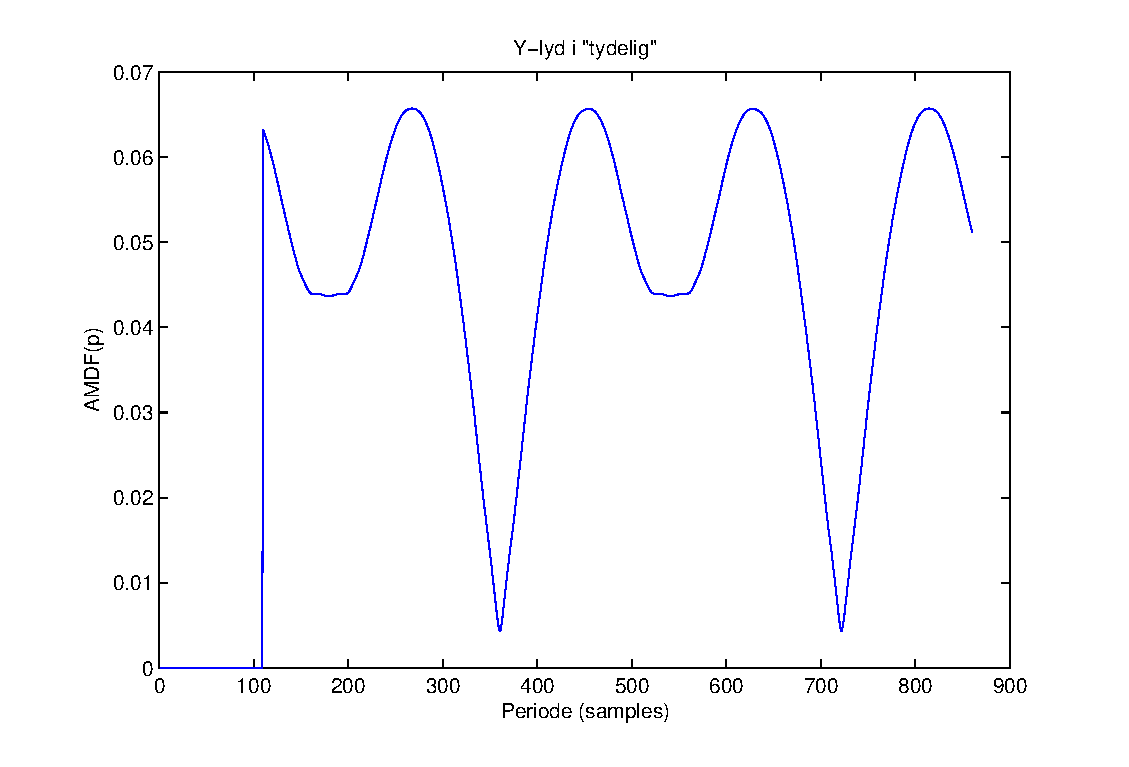
\includegraphics[width=120mm]{y-plot.eps}\\
\end{center}
\label{udstyr}
\caption{'Y'-lyd i 'tydelig'}
\end{figure}

Det ses at minimum ligger ved ca 730 samples, svarende til ca 60 Hz. Et lokalt minimum ses ved den dobbelte frekvens (den halve periode), hvilket formodentligt er en overtone.

Er den minimale v�rdi over et bestemt threshold, v�lger vi at opfatte frame'n som en ustemt lyd.

\subsection{Ustemte lyde}
I dette ekspempel analyseres 20 ms af 't'-lyden i 'tydeligt'. Det ses at alle v�rdier ligger forholdsvist samme sted p� y-aksen. Ingen v�rdi er under vores threshold og vi opfatter derfor frame'n som en ustemt lyd.

\begin{figure}
\begin{center}
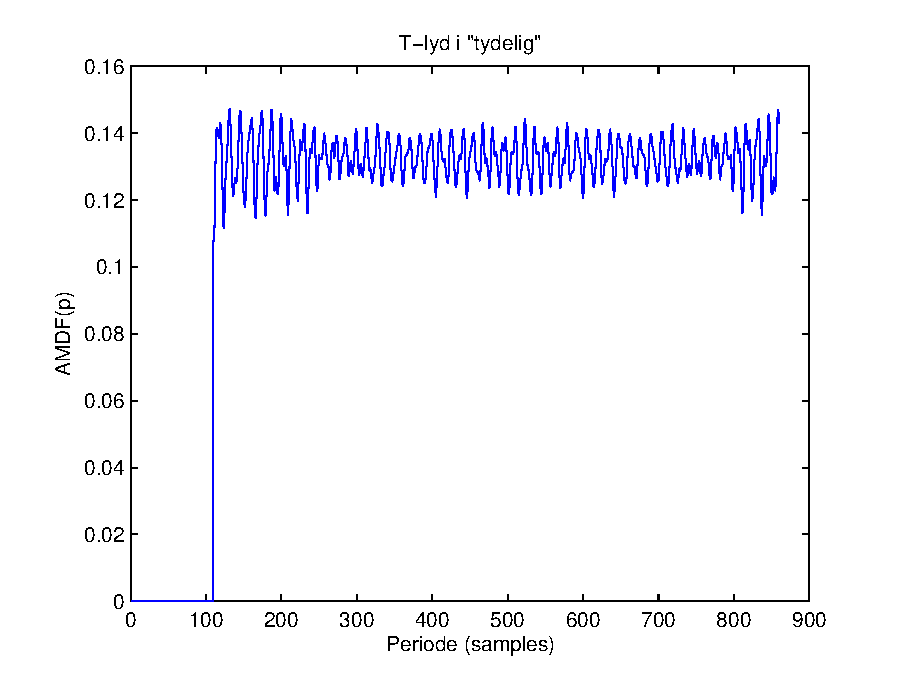
\includegraphics[width=120mm]{t-plot.eps}\\
\end{center}
\label{udstyr}
\caption{'T'-lyd i 'tydelig'}
\end{figure}


\section{Eksperimenter}
Vi �nsker at eksperimentere med forskellige vindue-st�rrelser, antallet af koefficienter, samt threshold'et for skelnen mellem stemt og ustemt lyd.

- pr�v med forsk. stemmelejer, eg. lys mandestemme (mikkel), m�rk mandestemme (bent/engl�nder), kvindestemme

- pr�v med forsk. vinduest�rrelser - beskriv evt. at vores vinduest�rrelse definerer den nederste pitch vi detecter (high\_sample = 0.7 * window\_size\_samples gennem eksperimentering)

- forsk. antal koefficienter

- pr�v med forsk. threshold for stemt/ustemt

Vi har i denne �velse lavet en succesfuld implementation af den kvantisering, som benyttes i JPEG. Vi har ogs� implementeret Huffman-encoding, prim�rt for at estimere komprimeringsfaktoren, men vores encoding kan ogs� udvides til at gemme billedet p� disken og senere decode det.

Vi har i vores program givet mulighed for at eksperimentere med kvantiseringen og f� vist resultatet, b�de grafisk samt i form af en PSNR v�rdi.


%\includeonly{filename,filename,...}

%Denne opgave er skrevet ved brug af \LaTeX2e
\end{document}
%*********************************************
%*                 end of                    *
%*              -=DOCUMENT=-                 *
%*********************************************
